%!TEX root = paper.tex

\section{Introduction}
\label{sec:intro}


Bayesian inference is an important technique to express hypothesis and
reason about data in data analytical tasks.  Today, many big data applications
are based on Bayesian inference. Examples include topic modeling
\cite{blei2003latent,Titov2008a}, sentiment analysis \cite{Titov2008b,
Jo2011,tsm}, spam filtering \cite{spam}, to name a few.


%One of most critical steps of Bayesian inference is to construct a
%\emph{probabilistic model} to formally represent the underlying 
%inference task \cite{cox}. The development of a probabilistic

%
%because a domain user may have to devise and
%implement many  different models before finding an appropriate one for
%a specific task. 

Bayesian inference is a complex process.
Consider a data scientist who wants to take into account the \emph{burstiness} 
of words when developing a new topic model.
She has to (i) define her own probabilistic graphical model 
(such as the one in \figref{fig:dcmlda}),
(ii) choose an appropriate inference algorithms (e.g., variational message
passing (VMP) \cite{vmp} or 
Gibbs sampling (GS) \cite{gibbs}),
(iii) handle the complex mathematics required by the algorithm (e.g., 
calculating the expectation of a complex distribution),
(iv) write the inference program that combines the model and 
the observations (the data that she has),
and (v) execute the inference program.
Existing scalable machine learning libraries such as MLlib 
 \cite{mllib} are of little help in this respect because they only
support popular models such as support vector machine (SVM), 
linear regression, latent Dirichlet allocation (LDA) \cite{blei2003latent}, etc.
 
In practice, a domain user may have to devise and
implement many  different models before finding an appropriate one 
for a specific task at hand. Unfortunately, Bayesian inference on big 
data requires extensive knowledge in both statistical
inference and programming techniques in distributed frameworks.
Different models or probability distributions call for varying
strategies for data and computation distribution.
Even though probabilistic models are theoretically compositional,
a large amount of boiler-plate code is often required.
Finally, model definitions, inference algorithms, and
data processing tasks are all mixed together in the resulting code,
making it hard to debug and reason about.

%For even a slight alteration to the model in quest of the most promising one,
%the model designer will have to re-derive the formulas and
%re-implement the inference codes, which is tedious and error-prone.


%
%Consider DCMLDA (see \figref{fig:dcmlda}), a non-standard model for topic
%modeling that accounts for burstiness in documents~\cite{Doyle2009}.
%\KZ{
%This model is different from standard LDA in that ...}
%None of the existing machine learning libraries including MLlib supports this
%model.

\begin{figure}[th]
\centering
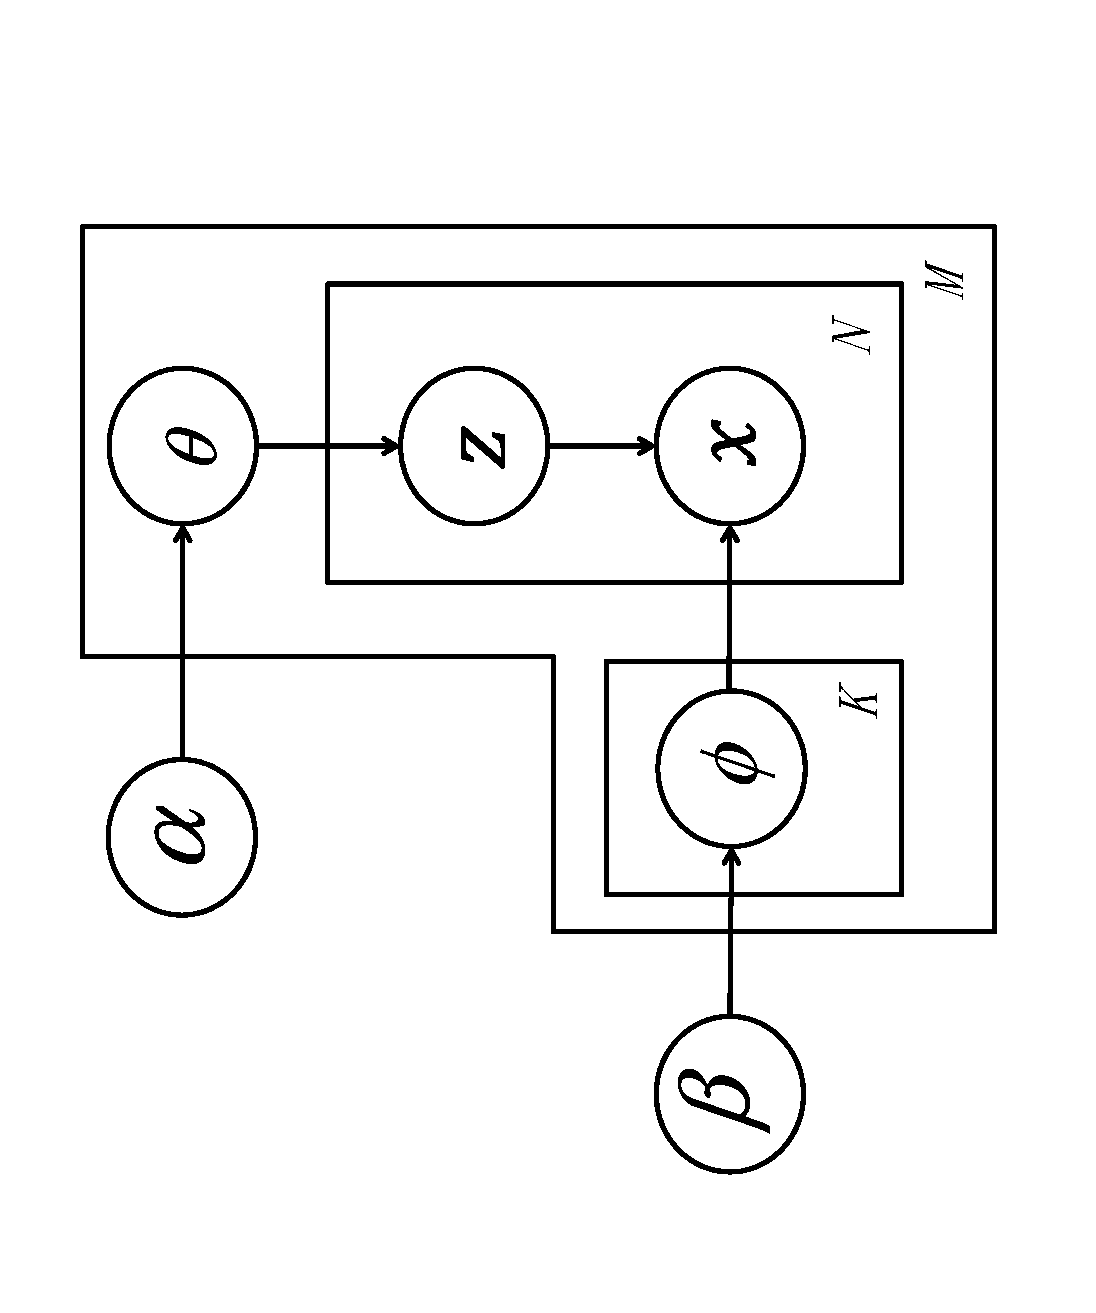
\epsfig{file=figs/DCMLDAintro.eps,width=0.6\columnwidth,angle=270}
\caption{DCMLDA, a probabilistic graphical model that is used as 
a topic model which accounts for word burstiness~\cite{Doyle2009}. 
which replace the multinomial distributions in standard latent 
Dirichlet allocation (LDA) by Dirichlet compound multionomial (DCM) 
distributions.  Although similar to LDA,
it is not supported by MLlib or any other standard machine learning
libraries because inference on DCMLDA typically requires
customization of the standard inference algorithm 
(e.g., re-derivation of formulas).
}
\label{fig:dcmlda}
\end{figure}

%To carry out statistical inference on DCMLDA with big data,
%the user has to implement inference algorithms such as
%Gibbs sampling~\cite{} or variational message passing (VMP)~\cite{}
%within a distributed framework, e.g.,
%Apache Spark \cite{Zaharia:2010:SCC:1863103.1863113} and Hadoop \cite{hadoop}.
%\figref{fig:dcmlda-code} shows part of the actually manually coded SPARK program
%implementing the VMP algorithm. \KZ{Give a little primer about VMP first. 
%Then explain this code a bit. Remember the reader
%might not know VMP or even PGM at all. So this explanation has to be very clear.
%Why this code can't be implemented as a library and why it's tedious to create this
%code. The following is not good enough!}
%\JL{VMP is a message passing algorithm which would pass messages between different nodes.}
%\YI{As it shown in line-4, it would take time for the lib to check the routing table and find the boundary number every time when we��re going to merge the message. For example, if we have $1500$ nodes and iterate for $40$ times then the lib would check the boundary for $60000$ times since each node would check its coming messages and check them, leading to a relatively huge overhead.}
%
%\begin{figure}[th]
%\begin{lstlisting}
%override def mergeImpl(msg: VertexAttr): Dirichlet = if (msg.isInstanceOf[Msg])
%      {
%        msg.asInstanceOf[Msg] match {
%          case (msg @ _) if (msg.srcId >=(228602L) && msg.srcId<(2824757L)) => {
%            val a = msg.asInstanceOf[DoubleArrayMsg].msg;
%            var i = 0;
%            while(SetCondition){
%              if (i<10)
%                {
%                  {
%                    this.alpha(i)+=(a(i));
%                    i = i+1
%                  };
%                  while(SetCondition)
%                }
%              else
%                ()
%            }
%          }
%          case _ => throw new Exception(StringContext("unknown msg from ", "").s(msg.asInstanceOf[Msg].srcId))
%        };
%        this
%      }
%\end{lstlisting}
%\caption{The SPARK code implementing VMP for DCMLDA model}
%\label{fig:dcmlda-code}
%\end{figure}
%
%
%%For even a slight alteration to the model in quest of the most promising one,
%%the model designer will have to re-derive the formulas and
%%re-implement the inference codes, which is tedious and error-prone.
%
%Custom models like DCMLDA~\cite{} are abundant in many data analytics tasks.
To address some of challenges with programmable and custom
probabilistic modeling,
an emerging paradigm called {\em probabilistic programming} was proposed
to unify programming with probabilistic modeling~\cite{pp}.
Languages in this paradigm can declaratively describe a probabilistic
model and systems were built to automatically generate inference code for
the model from the description.
%Probabilistic programming is an emerging
%paradigm that allows statistician and domain users to succinctly express a model
%definition within a host programming language and transfers the burden of
%implementing the inference algorithm from the user to the compilers and
%runtime systems \cite{pp}. For example, Infer.NET \cite{InferNET14} is a
%probabilistic programming framework that extends C\#.  The user can express,
%say, a Bayesian network in C\# and the compiler will generate code to perform
%inference on it. Such code could be as efficient as the implementation of
%the same inference algorithm carefully optimized by
%an experienced programmer.
%
So far, the emphasis of probabilistic programming has been put on the
expressiveness of the languages and the development of efficient inference
algorithms (e.g., Variational Message Passing \cite{vmp}, Gibbs sampling \cite{gibbs},
Metropolis-Hastings sampling \cite{mh}) to handle a wider range of probabilistic
models.  The issue of scaling out these frameworks, however, has hardly been
addressed.  For example, Infer.NET~\cite{InferNET14}, one of the most
mature probabilistic programming systems, only works on a single machine.
When we tried to use Infer.NET to train an LDA model of 96 topics and 9040-word
vocabulary on only 3\% of Wikipedia articles, the actual memory
requirement has already exceeded 512GB, larger than the amount of memory on
most commodity servers today.
%Frequent swapping makes each iteration take xxx hrs
%(still running, > 2 hr). Infer .NET deals with the scaling problem by
%splitting the whole dataset into chunks that fit in memory and iteratively
%load and process the chunks. Using the batched training, each iteration still
%takes over 21 minutes.

In this paper, we present InferSpark, a \emph{declarative Bayesian inference
framework} on top of Spark. It allows end users to succinctly {\em declare} a
 custom Bayesian network model using random variables, their prior
distributions as well as their inter-dependencies.
As such, even complex models can often be expressed with only a few 
lines of code.  The InferSpark system has modules 
that combine the model with the observations (the data),
prepare the complex mathematical input for the inference algorithm,
generate the corresponding efficient inference program,
and execute it on a Spark cluster of machines 
through a specialized runtime engine optimized for Bayesian inference.

%InferSpark compiler then takes the model description and generates
%appropriate parameterized inference code, which is instantiated at runtime
%by the input data and run efficiently on Spark distributed system.


%%%Bayesian networks form a dominant branch of probabilistic graphical models
%%%and include such popular models as naive Bayes, LDA, Bayes Point Machine (BPM)
%%%and Gaussian Mixture Model (GMM), as well as many other custom models~\cite{}.
%%%For example, \figref{fig:intro_lda_def} shows a 5-line InferSpark
%%%description of LDA.
%%%In contrast, it takes MLlib 503 lines of Scala code
%%%(excluding comments, javadocs, blank lines and utilities) to do the
%%%same job.
%and TSM~\cite{tsm}.


%The InferSpark project consists of two parts:
%\begin{packed_enum}
%	\item {\bf Extending Scala to support declarative modeling of
%	Bayesian networks}
%
%	Spark is implemented in Scala due to its functional nature.
%The fact that both preprocessing and post-processing can be
%included in one Scala program substantially eases the development process.
%	In InferSpark, we extend Scala with declarative constructs
%	while leveraging its functional features.
%	Carrying out statistical inference with InferSpark
%	is simple and intuitive, and implicitly enjoys the distributed computing
%	capability brought by Spark.  As an example, the LDA statistical model
%	was implemented using 503 lines of Scala code in MLlib
%	(excluding comments,
%	javadocs, blank lines, and utilities of MLlib).
%	With InferSpark, we could implement that using only 7 lines
%	of declarative code (see \figref{fig:intro_lda_def}).
%	
%
%	\item {\bf Building an InferSpark compiler and a runtime system}
%		
%	InferSpark compiles InferSpark models into Scala classes
%	and objects that implement the corresponding inference algorithms
%	with a set of API.
%	The user can call the API from their Scala programs to
%	specify the input (observed) data and query about the model
%	(e.g. compute the expectation of
%	some random variables or retrieve the parameters of the posterior
%	distributions). Meanwhile, the system provides interface for
%	algorithm developers to plugin new inference algorithms to support
%	new models.
%		
%\end{packed_enum}
%
%
%\begin{figure}
%\begin{lstlisting}
%@Model
%class LDA(K: Long, V: Long, alpha: Double, beta: Double){
%	val phi = (0L until K).map{_ => Dirichlet(beta, K)}
%	val theta = ?.map{_ => Dirichlet(alpha, K)}
%	val z = theta.map{theta => ?.map{_ => Categorical(theta)}}
%	val x = z.map{_.map{z => Categorical(phi(z))}}
%}
%\end{lstlisting}
%%@Model
%%class DCMLDA(K: Long, V: Long, alpha: Double, beta: Double) {
%%    val doc = for (i <- ?) yield {
%%        val phi = (0L until K).map(_ => Dirichlet(beta, V))
%%        val theta = Dirichlet(alpha, K)
%%        val z = ?.map(_ => Categorical(theta))
%%        val x = z.map(z => Categorical(phi(z)))
%%    }
%%}
%\label{fig:intro_lda_def}
%\caption{InferSpark Definition of LDA Model}
%\end{figure}

%Currently, InferSpark supports Bayesian network models. Bayesian network
%is a major branch of probabilistic graphical model and it has already covered
%models like naive Bayes, LDA, TSM \cite{tsm}, etc.
%The goal of this paper is to describe the workflow, architecture,
%and a preliminary implementation of
%InferSpark.  We will open-source InferSpark and support other models and
%inference algorithms afterwards.

To the best of our knowledge, InferSpark is the first endeavor to bring
probabilistic programming into the realm of (big) data engineering.
%InferSpark project aims to provide a scalable and
%extensible Bayesian inference system
%with a declarative interface to end-user. End-users can define Bayesian
%networks using a language embedded in Scala and let the compiler and runtime
%handle the Bayesian inference.
InferSpark is different from systems
for implementing inference algorithms such as MATLAB, R, SystemML
\cite{systemml}, which targets inference code developers instead of end-users.
It is also different from machine learning libraries such as Mahout
\cite{mahout}, MLlib \cite{mllib}, MADLib \cite{madlib}, which only support a
limited number of well-known models. When it comes to customized models, 
the users cannot use these libraries but have to write their own complex
inference code. 
InferSpark is similar to MLBase
\cite{mlbase} in the sense that they both provides end-users a declarative
interface but the latter mainly handles frequentists' approaches such as SVM
and logistic regressions.

\begin{figure}[th]
\centering
\includegraphics[width=0.7\columnwidth]{figs/DCMLDAmess1}
\caption{Message Passing Graph of DCMLDA}
\label{fig:dcmlda-mpg}
\end{figure}


Overall, InferSpark makes the following technical contributions:

\begin{description}
\item[Ease of modeling] InferSpark provides an expressive language, 
based on Scala, that can be used to describe customized, complex and 
composable Bayesian network models,
and to infer joint and posterior probabilities from these models. 
The model definition and user inference code are very succinct and 
are separated from one another. For example, the DCMLDA model could be
defined with just 7 lines of InferSpark code, while the corresponding
manually crafted Spark program that expresses and infers the model 
has more than 900 lines of code!
%\item[Inference code generation] We implement the mechanisms to automatically generate
%two popular inference algorithms, namely variational message pass (VMP)
%and Gibbs sampling (GS) from a large variety of models, to run on distributed SPARK environment.

\item[Distributed inference algorithms] 
InferSpark includes the distributed version of 
two popular serial inference algorithms, namely variational message passing
and Gibbs sampling. VMP supports Bayesian networks in the exponential
conjugate family while GS supports probabilistic graphical models with
conjugate distributions. Together these algorithms handle a wide range 
of probabilistic models including naive bayes, various types of
topic models, TSM~\cite{tsm}, GMM, etc.

\item[PGM-aware partitioning]
When running Bayesian inference on big data,
the inference process/algorithms actually needs to 
construct a huge graph called message passing graph (MPG), such as
the one in \figref{fig:dcmlda-mpg},
whose size is on par with the size of the given (observable) data.
Unlike most real world graphs,
the message passing graph 
does not follow the power law 
but largely follows the structure of its corresponding PGM (see \figref{fig:dcmlda}).
As a consequence,
InferSpark abandons the four generic vertex-cut 
graph partitioning strategies provided by Spark (GraphX),
which were designed for general real-world graphs,
but includes its own PGM-aware partitioning scheme.
Our thorough analysis
shows that while the existing vertex-cut 
graph partitioning strategies in GraphX
would result in
each vertex spans at $O(M)$ and $O(\sqrt{M})$ of the machines in a cluster of size $M$,
our PGM-aware vertex-cut partitioning strategy could result 
in $O(1)$ machines per vertex when applied to  message passing graphs.
As pointed out by \cite{graphX},
the communication and storage overhead of a vertex-cut graph processing system
is directly proportional to the sum of the number of machines spanned by each vertex,
our PGM-aware partitioning scheme can thus make the inference process 
substantially much more efficient.

\item[PGM-aware vertex-edge co-location]
General purpose graph processing engines like GraphX 
are {\bf not} in favor of co-locating the vertex information  ({\tt VertexRDD}) 
with the edge-set ({\tt EdgeRDD})
because a decent number of vertices would indeed appear in multiple 
machines' edge-set when facing real-world graphs.
However, with PGM-aware partitioning, InferSpark is able to 
evenly distribute the edge-set to multiple machines with 
%when each vertex spans only across $O(1)$ machines,
%that means 
most edges {\bf not} sharing vertices across machines.
As a consequence, InferSpark implements its own graph processing 
engine. The implementation adopts the APIs of GraphX for compatibility
but adopts a vertex-edge co-locating principle
to avoid unnecessary shuffling.
% incurred by the disjointness of 
%vertex and edge in a distributed setting.

%\item[Optimization over GraphX] Our runtime system is an improvement from the original GraphX engine.
%It supports checkpointing (to avoid long lineage), proper timing of caching and
%anti-caching (to improve efficiency under memory constraint),
% and partitioning (to avoid unnecessary replication and shuffling).
%\item[Scalable computation] Our experiments show InferSpark can (almost linearly) scale out and scale up on
%reasonably sized custom models and the standard LDA.
\end{description}

InferSpark is an open-source project.
New probability distributions and inference algorithms can all 
be added by the community.
InferSpark uses a plug-in architecture which makes it open-ended and adaptable.  
Whilst the existing implementation can support a wide range of models, 
there will always be cases where a new distribution type or algorithm is needed.
In this case, custom code can be written and freely mixed with 
the built-in functionality, minimizing the amount of extra work needed.
We have evaluated InferSpark using 
both custom models that not yet supported by any existing systems
and popular models preexisting in MLlib.
Our results show that InferSpark can express various custom models 
using just a few lines of code,
and the inference process can both scale-up and scale-out.


%\KZ{Need to expland the following technical challenges}
%\begin{enumerate}
%\item Most existing probabilistic programming platforms only implement sequential
% versions of inference algorithms such as variational message passing and Gibbs
% sampling, which means we cannot utilize the power of distributed computation. 
% Also for ease of use, we need to automatically generate parallel inference 
% code for custom probabilistic graphical models on Spark.
%\item GraphX only has two kinds of default partition strategies: hash and random,
% which do not gain much performance for inference problems in graphical models. 
% In order to speed up the inference, we override the default partition strategies 
% and implement partition strategies that proves more efficient than original ones.
%\item Excessive data replication and shuffling in GraphX making it hard to scale to large
%number of machines.
%\end{enumerate}
%


%
%For example, Bayesian inference algorithms are mostly iterative serial
%algorithms. When implementing them on Spark, we have to identify the
%parallelizable parts without violating the correctness of the algorithms and
%also adapt them to the computation model.
%% (\ZY{not the problem of
%%functional style. when updating a vertex $v$, $v$ needs to pull message from
%%neighbours $u$, and before the neighbours can return the message, they may
%%need to pull messages from their neighbours.
%%This translates to either 2 ``aggregate'' and 2
%%``join'', or 1 and 1 with cached message in GraphX.}).
%Furthermore,
%Spark is efficient for iterative machine learning algorithms
%that does not modify the in-memory RDD (e.g., Stochastic Gradient Descent in MLlib).
%%
%%because the data can reside in the memory as RDD,
%%
%%as long as the
%%data reside in the memory, especially for algorithms
%Statistical inference algorithms like VMP \cite{vmp}, however,
%require iteratively update the RDD.
%Therefore, the implementation requires persisting  the
%intermediate results before the first action of the next
%iteration to avoid unnecessary shuffling and
%unpersisting afterwards so that
%the memory consumption does not increase linearly with the number of iterations.
%It is also necessary to periodically checkpoint the RDD to avoid long lineage,
%which could overflow the memory and crash the program. \KZ{One might ask,
%is Spark the right choice to implement PP on, if there's so much difference
%between the intrinsic computation model of Spark and VMP?}

The remainder of this paper is organized as follows:
%Section \ref{sec:background} presents the essential background for this paper.
Section \ref{sec:related} discusses some related work.
Section \ref{sec:framework} then gives an overview of InferSpark.
%Section \ref{sec:implementation} gives the implementation details of InferSpark.
Section \ref{sec:optimization} presents the optimization specific to InferSpark.
Section \ref{sec:eval} presents an evaluation study of the current
version of InferSpark,
and Section \ref{sec:conclusion} contains our concluding remarks.



%Proper persisting,
%unpersisting and checkpointing is crucial to such iterative programs but are
%not easy to do in GraphX because not all combinations will work as it should.
%

%The iterative nature of
%inference algorithms is also a challenge because long running iterative
%programs on Spark could easily take excessively long to finish or even crash
%if the intermediate results are not properly persisted, unpersisted or
%checkpointed.
%We also have to deal with various compatibility issues among
%Spark, scala and JVM because our framework also makes use of several advanced
%features of scala.


%Despite availability of various statistical models, new models are constantly
%being proposed to adapt to different characteristics of the data. In the case
%of topic modeling, LDA is a widely used model but may still be outperformed
%by other topic models when used on different datasets.
%
%
%Nowadays, many new applications often
%call for various customized models, such as topic modelling
%
%The naive Bayes model is a simple classification model that has been
%successfully used in spam filtering and medical diagnosis.  In spam filtering,
%bag-of-word features are typically used. Each email is viewed as a set of words
%that appear at least once in it. The naive Bayes model assumes that the
%occurence of each word is independent and the probability of a spam email is
%simply the product of the probabilities of being a spam conditioned on each
%word. The conditional probabilities are inferred from a number of labeled
%emails. Given a new email, the trained model can give a probability of the
%email being spam.  When the probability is higher than some threshold, the
%email can be identified as a spam. Assigning zero probability to missing words
%in the training data could degrade the performance because any new email
%containing the missing word is assigned probability zero. Laplacian smoothing
%is used in such models to avoid giving zero probability to missing words in the
%training data.  Alternatively, adding a Beta prior to the parameters and
%performing Bayesian inference with the training data is equivalent to the
%laplacian smoothing. Besides the naive Bayes model, it is also possible use
%other classification models such as logistic regression and support vector
%machine.
%
%The latent Dirichlet allocation is a popular topic model. It is widely used to
%summarize topics from a lot of documents and to tag the documents with the
%topics. The LDA model describes a probabilitic generative process of the
%documents. With the documents as input, inference algorithm calculates the
%poseterior distribution of the parameters of the LDA model and generate lists
%of representative words for the topics. For example, it can produce lists of
%keywords for paper abstracts when trained with scientific papers. Meanwhile,
%from the posterior distribution computed by the inference algorithm, the most
%probable topics are assigned to the document.  The result can be used to
%categorize the papers according to their topics, saving a lot of manual labour.
%
%The LDA model is not the only choice of topic models. For example, the
%Sentence LDA model uses a sentence-level topic instead of per-word topic to
%capture the property that words in a sentence tend to share the same topic.
%The Dirichlet compound multinomial LDA \cite{Doyle2009} model uses differnt
%topic-word distributions in each document instead of a global one to account
%for the burstiness in a corpus.
%
%In online shopping sites, the users may express positive or negative feelings
%toward different aspects of a product (e.g. price, quality) in their comments,
%but it usually takes a lot of time for readers to obtain the information.
%Online shopping sites can use the sentiment and aspect information to collect
%feedbacks for improvement and allow users to quickly evaluate the products
%according to the senti-aspect keywords of others' comments. A lot of models
%such as the Topic Sentiment Model \cite{Mei2007}, the Multi-Grain LDA model
%\cite{Titov2008a}, the Aspect and Sentiment Unification Model \cite{Jo2011}
%and etc. are constantly proposed to extract the sentiment and aspect
%information from the user reviews.
%
%Despite avaliability of various statistical models, new models are constantly
%being proposed to adapt to different characteristics of the data. In the case
%of topic modelling, LDA is a widely used model but may still be outperformed
%by other topic models when used on different datasets. The development of
%models is not a easy task because the user may have to try differnt
%possibilities. For even a slight alteration to the existing model, the
%designer will have to re-derive the formulas and re-implement the inference
%algorithms.  Probabilistic programming allows the designer to simply write the
%model definition using a succint language and leave the inference task to the
%system, which offloads the burden of implementation and makes it much easier
%to evaluate a new model.
%
%Currently, most machine learning libraries (e.g. MLLib) only contain standard
%models like support vector machine, linear regression, latent Dirichlet
%allocation (LDA) and etc. To perform inference on customized models, the user
%has to implement his own algorithms instead of the off-the-shelf algorithms
%provided by the ML libraries. Developing inference code requires extensive
%knowledge in both Bayesian inference and programming techniques in distributed
%frameworks.  Moreover, model definition, inference algorithm and unrelated
%code are all mixed up in the resulting code, making it hard to debug and
%resaon about.

%\begin{figure*}[!th]
%	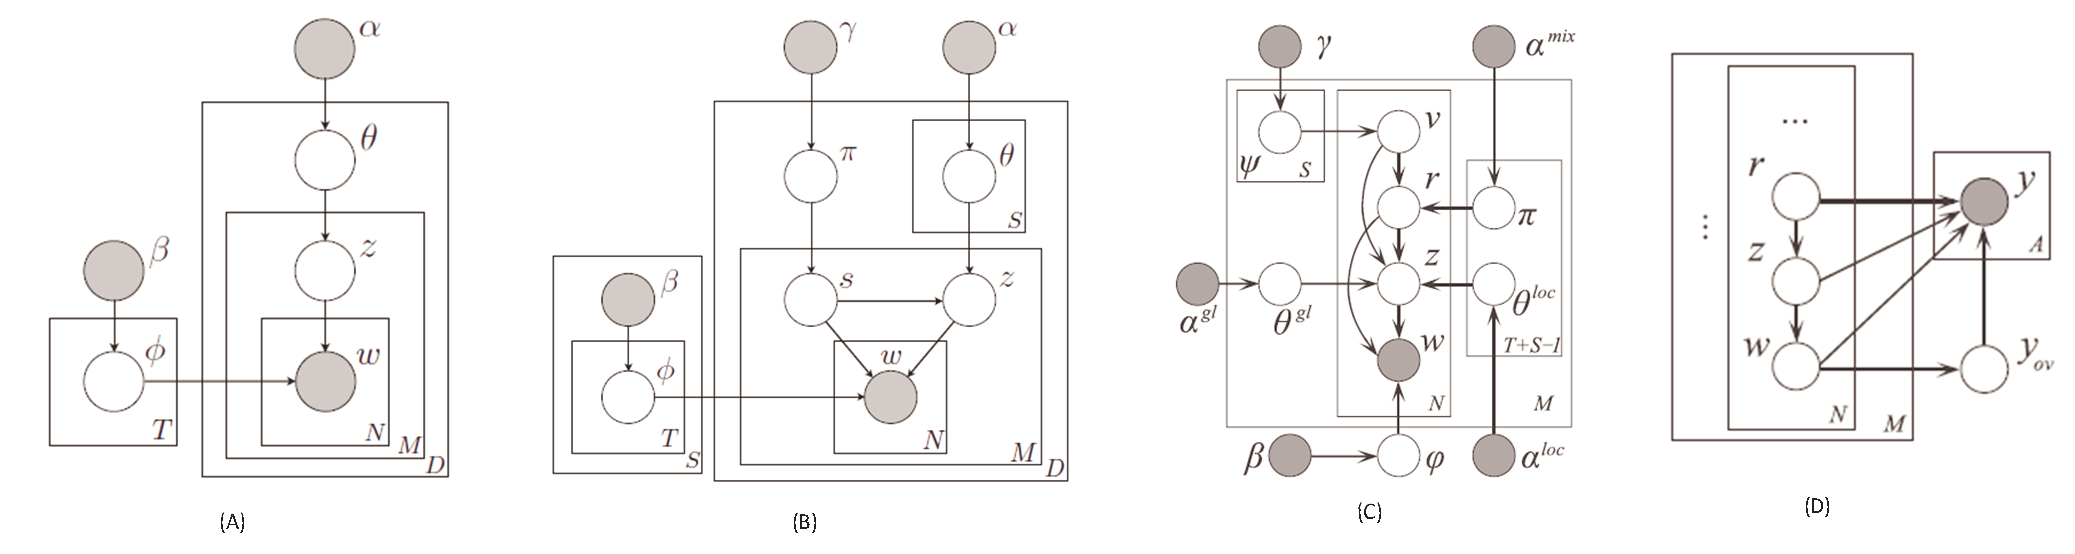
\includegraphics[scale=0.45]{figs/models.eps}
%	\caption{Different Bayesian networks: (A) Sentence-LDA for topic modelling
%	(B) Aspect and Sentiment Unification Model for sentiment analysis of reviews
%    (C) Multi-grained LDA model
%    (D) Multi-Aspect Sentiment model}
%	\label{fig:BNs}
%\end{figure*}


